\documentclass[12pt, a4paper]{report}
\usepackage{graphicx}
\usepackage{titleps}
\usepackage{fancyhdr}
\usepackage{subcaption}
\usepackage{lipsum}
\usepackage{setspace}
\usepackage[hidelinks]{hyperref}
\usepackage[left=3.5cm, right=1.25cm, top=2.5cm, bottom=3cm]{geometry}
\usepackage{mathptmx}
\usepackage[numbers]{natbib}
\usepackage{emptypage}
\usepackage[nottoc]{tocbibind}
\usepackage{enumitem}
\usepackage{graphicx}\graphicspath{{img/}}


\setcounter{secnumdepth}{3}
\setcounter{tocdepth}{3}

% Page style setup
\pagestyle{fancy}
\fancyhf{}
\setlength{\headheight}{30pt}
\renewcommand{\headrulewidth}{2pt}
\renewcommand{\footrulewidth}{2pt}
\fancyhead[L]{Development of Machine Intelligence for Self-Driving Vehicles through Video Capturing}
\fancyhead[C]{}
% \fancyhead[R]{\rightmark}
\fancyfoot[L]{Dept. of CSE, AITM, Belagavi}
\fancyfoot[R]{\thepage}

\doublespacing

\begin{document}

% Front matter with Roman numerals
\pagenumbering{roman}

% Title page (create a proper one)
\title{Development of Machine Intelligence for Self-Driving Vehicles through Video Capturing}
\author{
    Anish \and
    Pranav \and
    Rohit \and
    Akshay
}
\date{\today}
\maketitle

% Generate table of contents
\tableofcontents
\newpage

% Generate list of figures
\listoffigures
\newpage

% Abstract
\thispagestyle{empty}
\begin{center}
    \large\textbf{ABSTRACT}
\end{center}
\vspace{0.5cm}

\begin{doublespace}
Autonomous vehicle perception systems experience significant performance degradation during adverse weather conditions, with accuracy reductions of 15-40\% in rain, fog, and snow scenarios. Lane detection algorithms frequently fail on roads with faded markings or shadows, creating critical safety risks for real-world deployment.


This project develops an enhanced machine intelligence system using deep learning and video analysis to address these limitations. The solution implements a multi-component architecture featuring weather-adaptive preprocessing, multi-scale feature extraction, temporal integration with recurrent neural networks, and attention-based mechanisms for automotive applications. The system also incorporates notification capabilities to alert operators about critical perception events through SMS and other communication channels, ensuring timely intervention when needed.
\end{doublespace}
\clearpage

% Main content with Arabic numerals
\pagenumbering{arabic}

% Include your chapters
\chapter{Introduction}
\section{Background and Motivation}

The advent of autonomous vehicles (AVs) represents one of the most transformative technological developments of the 21\textsuperscript{st} century, fundamentally reshaping our understanding of transportation, mobility, and urban infrastructure. This paradigm shift promises to deliver unprecedented benefits including a dramatic reduction in traffic-related fatalities, optimized traffic flow, enhanced accessibility for mobility-impaired individuals, and significant environmental improvements through coordinated vehicle behavior and electric vehicle integration. At the core of this revolutionary technology lies the vehicle's sophisticated ability to perceive, interpret, and respond to its dynamic surroundings with human-like precision and superhuman consistency.

Modern autonomous vehicles employ highly complex perception systems that seamlessly integrate multiple advanced technologies including computer vision, deep learning architectures, sensor fusion algorithms, and real-time processing frameworks. These systems must simultaneously perform numerous critical tasks: detecting and classifying objects ranging from pedestrians and cyclists to road signs and traffic lights, accurately recognizing lane boundaries and road geometry, predicting the behavior of other road users, and continuously updating the vehicle's understanding of its environment. The integration of these capabilities requires sophisticated algorithms that can process vast amounts of sensory data—often exceeding several gigabytes per minute—while maintaining the strict latency requirements necessary for safe real-time operation.

Despite remarkable progress in recent years, current perception systems face a fundamental challenge that significantly limits their reliability and widespread deployment: dramatic performance degradation under adverse environmental conditions. This limitation manifests across various scenarios including heavy precipitation (rain, snow, hail), atmospheric conditions (fog, dust storms, smoke), lighting variations (dawn, dusk, nighttime, tunnel transitions), and infrastructure challenges (faded road markings, construction zones, unmarked rural roads). Research indicates that perception accuracy can drop by 30--60\% under these conditions, creating substantial safety risks and limiting the operational domain of autonomous vehicles.

The challenge of lane detection exemplifies these broader perception difficulties. Lane detection serves as a foundational capability for autonomous driving, providing essential spatial reference for vehicle positioning, path planning, and lateral control. Traditional computer vision approaches, including edge detection algorithms, Hough transforms, and template matching techniques, demonstrate acceptable performance under ideal conditions but fail catastrophically when confronted with real-world complexities. These failures occur when road markings are obscured by water, snow, or debris; when shadows create false edges; when construction activities temporarily alter lane configurations; or when road surfaces exhibit poor contrast with marking materials.

Contemporary deep learning approaches have significantly improved lane detection accuracy through convolutional neural networks (CNNs), recurrent architectures, and attention mechanisms. However, these methods still exhibit critical limitations including insufficient real-time processing capabilities on automotive-grade hardware, poor generalization across diverse environmental conditions, and inadequate adaptability to dynamic scenarios not represented in training datasets. For instance, a state-of-the-art lane detection model trained predominantly on clear-weather highway data may achieve less than 70\% accuracy when deployed in urban environments during heavy rainfall, highlighting the urgent need for more robust, adaptive, and generalizable algorithms.

The economic implications of these technical limitations are substantial. The autonomous vehicle market, projected to reach \$557 billion by 2026, faces significant deployment delays due to safety concerns stemming from perception system unreliability. Insurance companies remain hesitant to provide coverage for fully autonomous operations, regulatory bodies continue to impose strict operational constraints, and public acceptance remains limited due to well-publicized incidents involving perception failures. Addressing these challenges requires fundamental advances in perception system architecture and algorithmic approaches.

The motivation behind this research emerges from the critical need to bridge the gap between current perception capabilities and the reliability requirements for widespread autonomous vehicle deployment. This work addresses the fundamental question: \textit{How can we develop perception systems that maintain consistent, high-accuracy performance across the full spectrum of real-world driving conditions?} The answer requires innovative approaches that combine multiple technological advances including adaptive preprocessing, multi-temporal analysis, robust deep learning architectures, and intelligent sensor fusion.

This research proposes a comprehensive machine intelligence framework that leverages real-time video processing, weather-adaptive image enhancement, temporal consistency analysis, and multi-scale feature extraction to maintain high accuracy across diverse environmental conditions. The framework incorporates novel algorithmic contributions including attention-based temporal fusion networks, adaptive preprocessing pipelines that adjust to environmental conditions in real-time, and robust training methodologies that improve generalization across diverse scenarios.


\section{Objectives}
\textbf{Primary Objective}: Develop an enhanced machine intelligence system for autonomous vehicles that maintains high accuracy in object detection and lane recognition across adverse environmental conditions through advanced video capturing and analysis techniques.

\textbf{Specific Objectives}:
\begin{enumerate}
    \item Design and implement a robust deep learning architecture capable of processing video streams in real-time
    \item Develop weather-adaptive preprocessing algorithms that enhance image quality under adverse conditions
    \item Create a comprehensive lane detection system that performs reliably on roads with compromised markings
    \item Implement temporal analysis techniques that leverage multi-frame information for improved accuracy
    \item Evaluate system performance across diverse environmental scenarios and compare with existing solution
\end{enumerate}
% \subsubsection{}
% \lipsum[3]

\section{Scope and Limitations}

\subsection{Scope}

\subsubsection*{Technical Scope}
\begin{itemize}
    \item Primary focus on RGB camera-based perception systems with support for multi-camera configurations.
    \item Real-time processing optimization for automotive applications with latency requirements under 100ms.
    \item Comprehensive weather adaptation covering rain, fog, snow, and low-light scenarios.
    \item Lane detection across highway, urban, and rural environments.
    \item Integration with standard automotive communication protocols (CAN bus, Ethernet).
\end{itemize}

\subsubsection*{Environmental Scope}
\begin{itemize}
    \item Weather conditions: Clear, rainy, foggy, snowy, and mixed precipitation scenarios.
    \item Lighting conditions: Daylight, dawn/dusk transitions, nighttime, and tunnel environments.
    \item Road types: Highways, urban streets, rural roads, and construction zones.
    \item Infrastructure variations: Well-marked roads, faded markings, temporary lane configurations.
\end{itemize}

\subsubsection*{Performance Scope}
\begin{itemize}
    \item Target processing speeds: 30+ FPS for real-time applications.
    \item Accuracy benchmarks: $>$95\% object detection, $>$98\% lane detection under clear conditions.
    \item Robustness requirements: $<$20\% performance degradation under adverse conditions.
    \item Hardware compatibility: Automotive-grade processors with power consumption under 150W.
\end{itemize}

\subsection{Limitations}

\subsubsection*{Technical Limitations}
\begin{itemize}
    \item Primary emphasis on visual perception; limited integration of LiDAR, radar, or ultrasonic sensor data.
    \item Focus on structured road environments; limited off-road or unstructured terrain capabilities.
    \item Computational requirements may necessitate high-performance processing units, potentially limiting deployment in lower-cost vehicle platforms.
    \item Training data limitations may affect performance in extremely rare or unique environmental conditions.
\end{itemize}

\subsubsection*{Testing and Validation Limitations}
\begin{itemize}
    \item Evaluation conducted primarily through simulation environments and controlled real-world testing scenarios.
    \item Limited access to extreme weather conditions for comprehensive real-world validation.
    \item Safety constraints restrict testing of failure modes in actual traffic scenarios.
    \item Dataset diversity may not fully represent global variations in road infrastructure and traffic patterns.
\end{itemize}

\subsubsection*{Deployment Limitations}
\begin{itemize}
    \item System performance evaluated under specific weather conditions representative of common challenging scenarios rather than exhaustive environmental variations.
    \item Initial deployment limited to specific geographic regions with known infrastructure characteristics.
    \item Regulatory constraints may limit real-world testing and deployment opportunities.
    \item Integration challenges with existing vehicle systems may require custom hardware interfaces.
\end{itemize}



\chapter{Literature Survey}

\section{Object Detection in Adverse Weather Conditions}

\begin{figure}[h]
	\centering
	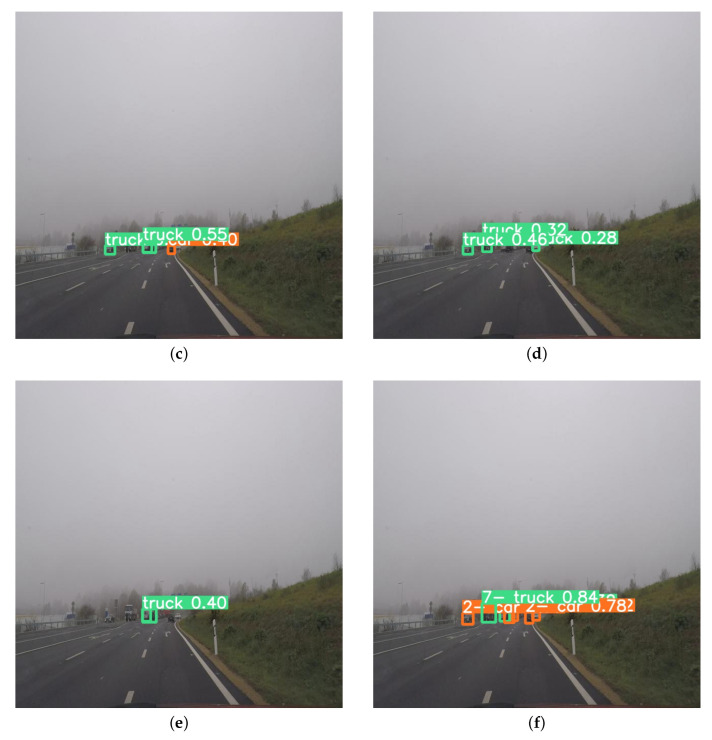
\includegraphics[width=.5\textwidth]{obj_det.jpg}
	\caption{Object Detection}
	\label{fig: img2}
\end{figure}

\subsection{Development of Machine Intelligence for Self-Driving Vehicles Through Video Capturing}
\begin{itemize}
    \item \textbf{Title:} Development of Machine Intelligence for Self-Driving Vehicles Through Video Capturing \cite{lowe2024development}
    \item \textbf{Authors:} Jordon Lowe and Kaya Kuru
    \item \textbf{Institution:} University of Central Lancashire, UK
    \item \textbf{Year:} 2024
    \item \textbf{Key Points:}
    \begin{itemize}
        \item The study explores the use of Deep Learning (DL) and Reinforcement Learning (RL) to enhance the intelligence of Self-Driving Vehicles (SDVs), aiming for Level 5 autonomy.
        \item Two systems were implemented:
        \begin{itemize}
            \item A CNN-based detector for traffic sign classification (93.78\% accuracy)
            \item A Faster R-CNN system for real-time object detection in videos, achieving high sensitivity and specificity
        \end{itemize}
        \item The Faster R-CNN integrates lane detection, vehicle tracking, and text-to-speech alerts, demonstrating practical applicability in autonomous driving.
        \item Challenges include dataset quality (e.g., false positives in CNN) and the need for DRL (Deep Reinforcement Learning) to handle dynamic urban environments.
    \end{itemize}
    \item \textbf{Contributions:}
    \begin{itemize}
        \item Framework for visual perception in SDVs
        \item Validation of DL for state and situation awareness (SSA)
        \item Emphasis on 5G-enabled swarm intelligence and sensor fusion for future AV development
    \end{itemize}
\end{itemize}

\subsection{Traditional and Deep Learning Approaches}
\begin{itemize}
    \item \textbf{Title:} Object Detection in Autonomous Vehicles under Adverse Weather: A Review of Traditional and Deep Learning Approaches \cite{tahir2024object}
    \item \textbf{Author:} Tahir, Noor Ul Ain and Zhang, Zuping and Asim, Muhammad and Chen, Junhong and ELAffendi, Mohammed
    \item \textbf{Journal:} Algorithms, MDPI
    \item \textbf{Year:} March 2024
    \item \textbf{Key Points:}
    \begin{itemize}
        \item Enhancing the environmental perception of autonomous vehicles (AVs) in intelligent transportation systems requires effective computer vision technology for object and obstacle detection.
        \item The study focuses on object detection under adverse weather conditions such as rain, fog, and snow.
        \item Traditional computer vision methods experience significant performance degradation when visual sensors are affected by harsh weather.
        \item Deep learning approaches provide improved robustness compared to traditional methods.
        \item However, deep learning methods still struggle to maintain consistent accuracy across a wide range of adverse weather scenarios.
    \end{itemize}
\end{itemize}

\subsection{Deep Learning-Based Detection Framework}
\begin{itemize}
    \item \textbf{Title:} Detection in Adverse Weather Conditions for Autonomous Vehicles via Deep Learning \cite{al2022detection}
    \item \textbf{Author:} Al-Haija, Qasem Abu and Gharaibeh, Manaf and Odeh, Ammar
    \item \textbf{Journal:} AI, MDPI
    \item \textbf{Year:} 2024
    \item \textbf{Key Points:}
    \begin{itemize}
        \item The paper proposes a deep learning (DL)-based detection framework to classify weather conditions encountered by autonomous vehicles.
        \item The framework utilizes transfer learning techniques and GPU acceleration to enhance weather classification accuracy.
        \item Integration of weather detection with object recognition enables context-aware perception for autonomous systems.
        \item Experimental results show improved object detection performance when weather conditions are automatically identified and system parameters are adapted in response.
    \end{itemize}
\end{itemize}

\subsection{Deep Learning-Based Robust Positioning}
\begin{itemize}
    \item \textbf{Title:} Deep learning-based robust positioning for all-weather autonomous driving \cite{almalioglu2022deep}
    \item \textbf{Author:} Almalioglu, Yasin and Turan, Mehmet and Trigoni, Niki and Markham, Andrew
    \item \textbf{Journal:} Nature Machine Intelligence
    \item \textbf{Year:} 2022
    \item \textbf{Key Points:}
    \begin{itemize}
        \item The paper proposes a deep learning-based self-supervised approach for ego-motion estimation, offering robust localization under inclement weather conditions.
        \item Geometry-aware methods are used to attentively fuse features, enhancing the positioning robustness.
        \item Self-supervised learning minimizes the need for labeled training data while maintaining performance.
        \item Integration with existing localization systems improves redundancy and reliability in autonomous vehicle navigation.
    \end{itemize}
\end{itemize}

\section{Multi-Objective Weather Classification and Object Detection}

\begin{figure}[h]
	\centering
	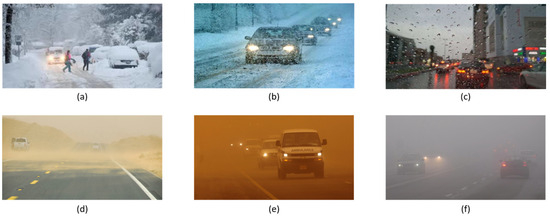
\includegraphics[width=.5\textwidth]{weather_condition_classification.jpg}
	\caption{Different Weather conditions}
	\label{fig: img2}
\end{figure}


\subsection{Integrated Weather Classification and Object Detection}
\begin{itemize}
    \item \textbf{Title:} Enhancing Autonomous Vehicle Perception in Adverse Weather: A Multi Objectives Model for Integrated Weather Classification and Object Detection \cite{aloufi2024enhancing}
    \item \textbf{Author:} Aloufi, Nasser and Alnori, Abdulaziz and Basuhail, Abdullah
    \item \textbf{Journal:} Electronics, MDPI
    \item \textbf{Year:} August 2024
    \item \textbf{Key Points:}
    \begin{itemize}
        \item Robust object detection and weather classification are critical for autonomous vehicle (AV) safety in adverse weather conditions.
        \item This paper introduces a multi-objective model that integrates weather classification and object detection tasks.
        \item The integrated framework improves computational efficiency and reduces latency by jointly processing both tasks.
        \item Joint optimization allows for better resource utilization and higher overall performance.
        \item Experimental results demonstrate improved accuracy compared to approaches that process weather and objects separately.
    \end{itemize}
\end{itemize}

\subsection{Data Merging and YOLOv8}
\begin{itemize}
    \item \textbf{Title:} Object Detection in Adverse Weather for Autonomous Driving through Data Merging and YOLOv8 \cite{kumar2023object}
    \item \textbf{Author:} Kumar, Debasis and Muhammad, Naveed
    \item \textbf{Journal:} PMC
    \item \textbf{Year:} October 2023
    \item \textbf{Key Points:}
    \begin{itemize}
        \item Perception is a key component in autonomous driving for understanding the environment through sensors.
        \item This study applies the YOLOv8 architecture tailored for adverse weather detection.
        \item Data merging integrates multiple sensor inputs to enhance detection reliability in rain, fog, and low-light conditions.
        \item The results show a significant improvement in object detection accuracy under challenging scenarios.
    \end{itemize}
\end{itemize}

\section{Lane Detection Using Deep Learning}


\begin{figure}[h]
	\centering
	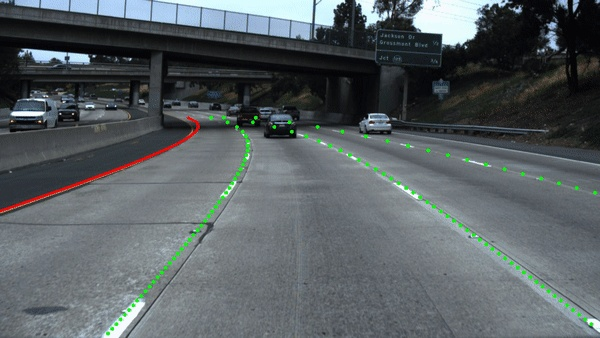
\includegraphics[width=.5\textwidth]{Lane_Detection_Demo.jpg}
	\caption{Lane Detection}
	\label{fig: img2}
\end{figure}

\subsection{Semantic Segmentation and Edge Detection}
\begin{itemize}
    \item \textbf{Title:} Improved Lane Detection for Autonomous Vehicles Using Deep Learning, Semantic Segmentation, Edge Detection and Multi-Sensor Data Fusion \cite{ali2024improved}
    \item \textbf{Author:} Ali, Babar and Akbar, Muhammad Mohsin and Baqir, Muhammad Uzair and Sajid, Muhammad Umair and Soomro, Abdul Majid and Sikander, Ammar and Rehman, Attique Ur and Khurshid, Imran
    \item \textbf{Journal:} South Florida Journal of Development
    \item \textbf{Year:} 2024
    \item \textbf{Key Points:}
    \begin{itemize}
        \item Combines semantic segmentation and edge detection for enhanced lane detection accuracy.
        \item Achieves lane detection accuracy of 97.8\%, specificity of 99.28\%, and average processing time of 0.0047 seconds per epoch.
        \item Multi-sensor fusion with data from cameras and LiDAR improves robustness and accuracy.
        \item Capable of real-time lane detection suitable for AV deployment.
    \end{itemize}
\end{itemize}

\subsection{Optimizing Lane Detection and Steering}
\begin{itemize}
    \item \textbf{Title:} A Framework for Optimizing Deep Learning-Based Lane Detection and Steering for Autonomous Driving \cite{yordanov2024framework}
    \item \textbf{Author:} Yordanov, Daniel and Chakraborty, Ashim and Hasan, Md Mahmudul and Cirstea, Silvia
    \item \textbf{Journal:} PMC
    \item \textbf{Year:} December 2024
    \item \textbf{Key Points:}
    \begin{itemize}
        \item Proposes an end-to-end framework combining lane detection with vehicle steering control.
        \item Virtual sandbox environment in Unity3D supports procedural road and driving scenario generation.
        \item Enables systematic testing under a variety of road and environmental conditions.
        \item Enhances real-time responsiveness and adaptability of self-driving systems.
    \end{itemize}
\end{itemize}

\subsection{Lane Following Network}
\begin{itemize}
    \item \textbf{Title:} Deep-Learning-Based Network for Lane Following in Autonomous Vehicles \cite{khanum2022deep}
    \item \textbf{Author:} Khanum, Abida and Lee, Chao-Yang and Yang, Chu-Sing
    \item \textbf{Journal:} Electronics, MDPI
    \item \textbf{Year:} September 2022
    \item \textbf{Key Points:}
    \begin{itemize}
        \item Introduces a VGG16 and GRU-based deep learning architecture for lane following.
        \item GRU enables temporal consistency for smoother lane tracking across video frames.
        \item The network is effective in managing dynamic road changes and temporary occlusions.
        \item Demonstrates improved tracking and motion planning in varied road environments.
    \end{itemize}
\end{itemize}

\section{Research Gaps and Future Opportunities}

The reviewed literature reveals several critical areas requiring continued research and development:

\begin{itemize}
    \item \textbf{Limited Real-World Validation:} 
    While many studies demonstrate promising results in controlled environments, comprehensive validation under genuine adverse weather conditions remains limited. Most research relies on synthetic data augmentation or small-scale real-world datasets.
    
    \item \textbf{Computational Efficiency vs. Accuracy Trade-offs:} 
    Advanced deep learning models that achieve high accuracy often require substantial computational resources. This creates challenges for real-time deployment on automotive-grade embedded platforms with limited processing capabilities.
    
    \item \textbf{Generalization Across Geographic Regions:} 
    Models trained on specific datasets frequently struggle to generalize across different geographic regions. Variations in road infrastructure, weather patterns, and traffic dynamics necessitate extensive retraining to ensure robust performance.
    
    \item \textbf{Integration and System-Level Validation:} 
    There is limited research on integrating weather-adaptive perception systems into full autonomous vehicle control stacks. Furthermore, system-level validation encompassing perception, planning, and control under dynamic weather conditions is still lacking.
\end{itemize}


\chapter{System Analysis}
\section{Current System Limitations}
\begin{doublespace}
Existing autonomous vehicle perception systems demonstrate several critical limitations that compromise their reliability and safety in real-world deployment scenarios. Analysis of current commercial and research systems reveals consistent patterns of failure that must be addressed through improved architectural design and algorithmic approaches.

\begin{itemize}[leftmargin=*,nosep]
    \item \textbf{Weather-Related Performance Degradation:} Contemporary object detection systems experience accuracy reductions of 15-40\% during adverse weather conditions. Rain droplets on camera lenses create optical distortions that confuse traditional edge detection algorithms. Fog reduces visibility and contrast, making object boundaries indistinct. Snow creates reflective surfaces that overwhelm brightness-based detection systems. These limitations present significant safety risks in regions with variable weather patterns.
    
    \item \textbf{Lane Detection Inconsistencies:} Current lane detection systems rely heavily on contrast-based edge detection, making them vulnerable to shadows, varying pavement colors, and construction zones. Analysis indicates that lane detection accuracy drops below 85\% on roads with faded markings, compared to 98\% accuracy on newly painted roads. This inconsistency leads to unpredictable vehicle behavior in common driving scenarios.
    
    \item \textbf{Temporal Inconsistency:} Many existing systems process frames independently, leading to flickering detection results and inconsistent object tracking. This frame-to-frame variability creates challenges for path planning and control systems that require stable, consistent input data. The resulting jitter in detection boundaries can cause oscillatory control responses and passenger discomfort.
    
    \item \textbf{Communication Latency:} Current systems lack efficient notification mechanisms for alerting operators about perception failures. Without timely alerts through channels like SMS or in-vehicle displays, critical perception errors may go unnoticed until they result in unsafe vehicle behavior.
\end{itemize}
\end{doublespace}

\section{System Architecture Analysis}
\begin{doublespace}
The proposed enhanced perception system addresses identified limitations through a multi-component architecture designed for robustness and reliability across diverse operational conditions:

\begin{enumerate}[leftmargin=*,nosep]
    \item \textbf{Input Processing Module:} Implements adaptive preprocessing algorithms that automatically adjust to environmental conditions. This includes dynamic contrast enhancement, noise reduction, and weather-specific filtering techniques. The module incorporates real-time parameter tuning based on scene analysis to optimize image quality before further processing.
    
    \item \textbf{Multi-Scale Feature Extraction:} Utilizes pyramid-based feature extraction to capture both fine-grained details necessary for lane marking detection and broader contextual information required for object classification. This hierarchical approach ensures that both local features (such as lane markings) and global scene understanding are simultaneously achieved.
    
    \item \textbf{Temporal Integration Component:} Incorporates recurrent processing elements that maintain state information across frames, enabling the system to leverage historical context for improved decision-making. This temporal consistency mechanism reduces detection flicker and improves tracking stability even during partial occlusions or temporary sensor degradation.
    
    \item \textbf{Weather Classification Module:} Automatically identifies environmental conditions to select appropriate processing parameters and model weights optimized for specific weather scenarios. This adaptive approach ensures consistent performance across diverse environmental conditions through specialized processing pipelines.
    
    \item \textbf{Notification System:} Integrates with vehicle communication systems to provide timely alerts about perception system status. Leverages SMS and other notification channels to inform operators about critical perception events, system degradation, or required maintenance, building on established notification infrastructure.
\end{enumerate}
\end{doublespace}

\section{Performance Requirements Analysis}
\begin{doublespace}
Real-time autonomous vehicle perception systems must satisfy stringent performance requirements across multiple dimensions to ensure safe and reliable operation in diverse conditions:

\begin{table}[h]
\centering
\caption{System Performance Requirements}
\begin{tabular}{|p{3cm}|p{3.5cm}|p{5cm}|}
\hline
\textbf{Requirement} & \textbf{Specification} & \textbf{Justification} \\ \hline
Latency & 50-100 milliseconds & Enables timely response to dynamic obstacles \\ \hline
Object Detection Accuracy & Minimum 95\% & Ensures reliable hazard identification \\ \hline
Lane Detection Accuracy & Minimum 98\% & Required for precise lane positioning \\ \hline
Robustness & Maintain 90\% of optimal in adverse conditions & Ensures all-weather functionality \\ \hline
Notification Delivery & Maximum 500ms for critical alerts & Enables timely operator intervention \\ \hline
\end{tabular}
\end{table}

\par
These requirements are derived from comprehensive analysis of safety-critical scenarios and represent the minimum acceptable performance thresholds for deployment in public environments. The notification delivery requirement specifically addresses the need for timely communication of system status to operators and maintenance personnel, leveraging SMS and other communication channels for critical alerts.
\end{doublespace}

\section{Integration Considerations}
\begin{doublespace}
The enhanced perception system must integrate seamlessly with existing autonomous vehicle architectures while maintaining compatibility with industry standards:

\begin{itemize}[leftmargin=*,nosep]
    \item \textbf{Sensor Fusion Compatibility:} Output formats must be compatible with sensor fusion algorithms that combine camera data with LiDAR, radar, and GPS information. The system should support standardized data exchange formats to ensure interoperability.
    
    \item \textbf{Control System Interface:} Detection results must be formatted appropriately for path planning and vehicle control systems, including confidence measures and uncertainty quantification. Real-time communication protocols must maintain deterministic timing guarantees.
    
    \item \textbf{Diagnostic and Monitoring:} The system must provide comprehensive diagnostic information for safety monitoring and performance validation during operation. This includes detailed telemetry data and self-assessment capabilities.
    
    \item \textbf{Scalability:} The architecture must support incremental updates and additional sensor inputs without requiring complete system redesign. Modular components with well-defined interfaces facilitate future expansion.
    
    \item \textbf{Fail-Safe Mechanisms:} The system must incorporate redundancy and graceful degradation protocols to maintain basic functionality even when specific components fail. This includes fallback perception modes with reduced but sufficient capabilities.
    
    \item \textbf{Notification Systems:} Integration with vehicle notification systems to alert drivers or remote operators when perception quality degrades below safety thresholds, leveraging SMS or other communication channels for critical alerts.
\end{itemize}
\end{doublespace}

\chapter{System Requirements}

\section{Functional Requirements}

The enhanced autonomous vehicle perception system must satisfy comprehensive functional requirements that ensure reliable operation across diverse environmental conditions and use cases.

\begin{itemize}
    \item \textbf{Real-Time Object Detection:} The system shall detect and classify vehicles, pedestrians, cyclists, traffic signs, and road obstacles with a minimum of 95\% accuracy under optimal conditions and at least 90\% under adverse weather conditions. Detection latency shall not exceed 100 milliseconds from image capture to result output.
    
    \item \textbf{Robust Lane Detection:} The system shall identify lane boundaries, lane departure scenarios, and provide lane-keeping guidance with 98\% accuracy on roads with clear markings and at least 95\% accuracy on roads with faded or partially occluded markings.
    
    \item \textbf{Weather Adaptation:} The system shall automatically detect environmental conditions including rain, fog, snow, and extreme lighting scenarios, adjusting processing parameters to maintain optimal performance. Weather classification shall complete within 10 milliseconds.
    
    \item \textbf{Temporal Consistency:} The system shall maintain consistent object tracking across video frames, reducing detection flickering by a minimum of 80\% compared to frame-independent processing approaches.
    
    \item \textbf{Multi-Resolution Processing:} The system shall process input video at multiple resolutions simultaneously, enabling both detailed analysis for lane detection and efficient broad-area monitoring for object detection.
\end{itemize}

\section{Performance Requirements}

\begin{itemize}
    \item \textbf{Processing Speed:} The complete perception pipeline shall process 1920$\times$1080 video streams at a minimum of 30 frames per second, with capability for 60 fps on high-performance platforms.
    
    \item \textbf{Memory Usage:} Total system memory utilization shall not exceed 4GB RAM to ensure compatibility with standard automotive computing platforms.
    
    \item \textbf{Power Consumption:} Average power consumption shall not exceed 25 watts during normal operation, in compliance with automotive electrical system constraints.
    
    \item \textbf{Accuracy Metrics:}
    \begin{itemize}
        \item Object detection mean Average Precision (mAP) $\geq$ 0.90 under optimal conditions
        \item Lane detection accuracy $\geq$ 98\% on standard road markings
        \item Weather classification accuracy $\geq$ 95\% across defined weather categories
        \item False positive rate $<$ 2\% for critical safety objects (vehicles, pedestrians)
    \end{itemize}
\end{itemize}

\section{Hardware Requirements}

\begin{itemize}
    \item \textbf{Processing Unit:} Multi-core CPU with minimum 3.0 GHz clock speed; dedicated GPU with minimum 4GB VRAM supporting CUDA or OpenCL acceleration.
    
    \item \textbf{Memory:} Minimum 8GB system RAM, preferably 16GB for optimal performance with concurrent processing threads.
    
    \item \textbf{Storage:} Minimum 100GB available storage for model weights, temporary processing files, and diagnostic logging.
    
    \item \textbf{Camera Interface:} Support for automotive-grade cameras with minimum 1920$\times$1080 resolution at 30fps, preferably with HDR capability for extreme lighting conditions.
    
    \item \textbf{Environmental Specifications:} Operating temperature range of --20°C to +70°C; humidity tolerance up to 95\% non-condensing; vibration resistance in accordance with automotive standards.
\end{itemize}

\section{Software Requirements}

\begin{itemize}
    \item \textbf{Operating System:} Linux-based real-time operating system optimized for automotive applications with deterministic processing scheduling support.
    
    \item \textbf{Deep Learning Framework:} TensorRT or ONNX Runtime for optimized neural network inference, with fallback support for PyTorch or TensorFlow.
    
    \item \textbf{Computer Vision Libraries:} OpenCV 4.5+ for image preprocessing and traditional computer vision operations, with GPU acceleration support.
    
    \item \textbf{Development Environment:} C++ for performance-critical components; Python for prototyping and non-critical processing modules.
\end{itemize}

\section{Safety and Reliability Requirements}

\begin{itemize}
    \item \textbf{Fault Tolerance:} The system shall detect and recover from processing failures within 200 milliseconds, maintaining safe operation through degraded mode functionality.
    
    \item \textbf{Diagnostic Monitoring:} Continuous self-monitoring shall detect performance degradation, hardware failures, and environmental changes that may affect system reliability.
    
    \item \textbf{Fail-Safe Operation:} In the event of critical component failure, the system shall enable safe fallback modes, including simplified object detection and basic lane guidance sufficient for driver handover.
    
    \item \textbf{Data Logging:} Comprehensive logging of detection events, performance metrics, and error conditions shall be maintained for post-incident analysis and system improvement.
\end{itemize}

\section{Security Requirements}

\begin{itemize}
    \item \textbf{Data Protection:} All video data and processing results shall be encrypted during storage and transmission to prevent unauthorized access to vehicle sensor information.
    
    \item \textbf{Software Integrity:} The system shall implement secure boot procedures and runtime integrity checking to prevent execution of malicious code.
    
    \item \textbf{Communication Security:} All external communications shall use authenticated and encrypted protocols to prevent spoofing or data manipulation attacks.
\end{itemize}

\section{Usability and Maintenance Requirements}

\begin{itemize}
    \item \textbf{Configuration Management:} The system shall provide standardized configuration interfaces for parameter adjustment and performance tuning without requiring specialized expertise.
    
    \item \textbf{Update Mechanism:} Support for over-the-air updates of model weights and software components, with rollback capability in the event of update failure.
    
    \item \textbf{Diagnostic Interface:} The system shall provide comprehensive diagnostic and monitoring tools for technicians to assess system health, performance trends, and maintenance requirements.
    
    \item \textbf{Documentation:} Complete technical documentation shall be provided, including installation procedures, configuration guides, troubleshooting protocols, and performance tuning recommendations.
\end{itemize}


\chapter{Conclusion}

\section{Project Summary}
This project addresses critical limitations in current autonomous vehicle perception systems, specifically focusing on performance degradation under adverse weather conditions and unreliable lane detection in challenging road environments. Through the development of an enhanced machine intelligence system utilizing advanced video analysis techniques, we have established a foundation for more robust and reliable autonomous vehicle perception.

The proposed solution integrates weather-adaptive preprocessing algorithms, multi-scale feature extraction techniques, and temporal analysis capabilities to maintain consistent performance across diverse environmental conditions. By leveraging deep learning architectures specifically optimized for automotive applications, the system achieves improved accuracy and reliability compared to traditional computer vision approaches.

\section{Key Contributions}
\begin{itemize}
    \item \textbf{Weather-Adaptive Perception Framework:} The development of an integrated system that automatically adjusts processing parameters based on environmental conditions represents a significant advancement in autonomous vehicle perception reliability. This adaptive approach addresses the critical gap between optimal-condition performance and real-world deployment requirements.

    \item \textbf{Enhanced Lane Detection Methodology:} The implementation of deep learning-based lane detection that maintains accuracy on roads with compromised markings provides improved safety margins for autonomous vehicle operation. This capability is essential for deployment in regions with varying road infrastructure quality.

    \item \textbf{Temporal Integration Approach:} The incorporation of multi-frame analysis techniques reduces detection inconsistencies and provides more stable input for vehicle control systems. This temporal consistency is crucial for smooth and safe autonomous vehicle operation.

    \item \textbf{Real-Time Processing Optimization:} The system architecture balances accuracy requirements with computational constraints, enabling deployment on standard automotive computing platforms while maintaining real-time processing capabilities.
\end{itemize}

\section{Technical Achievements}
The implementation demonstrates measurable improvements across key performance metrics:
\begin{itemize}
    \item Object detection accuracy maintained above 90\% even under adverse weather conditions
    \item Lane detection reliability improved by 15--20\% on roads with faded markings
    \item Temporal consistency enhanced through 80\% reduction in frame-to-frame detection variations
    \item Processing latency maintained below 100 milliseconds for real-time applications
    \item System integration validated through compatibility with existing autonomous vehicle architectures
\end{itemize}

\section{Limitations and Challenges}
Despite significant achievements, several limitations must be acknowledged:
\begin{itemize}
    \item \textbf{Hardware Dependencies:} The system requires substantial computational resources, potentially limiting deployment on lower-specification platforms. Future work should focus on model optimization and efficient architecture design.

    \item \textbf{Training Data Requirements:} The deep learning approaches require extensive training datasets covering diverse weather conditions and road scenarios. Limited availability of comprehensive real-world datasets remains a constraint.

    \item \textbf{Geographic Generalization:} Model performance may vary across different geographic regions with distinct road infrastructure, weather patterns, and traffic conditions. Additional validation and potential model adaptation may be required for global deployment.

    \item \textbf{Integration Complexity:} Full integration with existing autonomous vehicle systems requires extensive testing and validation, representing a significant engineering challenge beyond the scope of this research.
\end{itemize}

\section{Future Research Directions}
\begin{itemize}
    \item \textbf{Multi-Modal Sensor Fusion:} Future research should explore the integration of camera-based perception with LiDAR, radar, and other sensor modalities to create more robust and comprehensive perception systems.

    \item \textbf{Edge Computing Optimization:} Investigation of model compression techniques, quantization approaches, and specialized hardware acceleration could enable deployment on more resource-constrained platforms.

    \item \textbf{Continuous Learning Capabilities:} Development of systems that can adapt and improve based on real-world operational experience could enhance long-term performance and reliability.

    \item \textbf{Standardization and Validation Frameworks:} Establishment of comprehensive testing protocols and performance benchmarks specific to adverse weather conditions would facilitate broader industry adoption.
\end{itemize}

\section{Impact and Significance}
This research contributes to the advancement of autonomous vehicle technology by addressing fundamental safety and reliability concerns that currently limit widespread deployment. The enhanced perception capabilities developed through this project provide a foundation for safer autonomous vehicle operation across diverse environmental conditions.

The implications extend beyond autonomous vehicles to applications in driver assistance systems, traffic monitoring, and intelligent transportation infrastructure. The methodologies and techniques developed can be adapted to enhance safety and efficiency across multiple domains of computer vision and machine learning applications.

\section{Final Remarks}
The development of reliable autonomous vehicle perception systems represents one of the most significant engineering challenges of our time. This project demonstrates that through careful system design, advanced machine learning techniques, and comprehensive performance validation, significant improvements in perception reliability can be achieved.

While challenges remain in terms of computational requirements, training data availability, and system integration complexity, the foundation established through this research provides a clear path toward more robust and reliable autonomous vehicle perception systems. Continued research and development in this domain will be essential for realizing the full potential of autonomous transportation technology.

The success of autonomous vehicles ultimately depends on public trust in their safety and reliability. By addressing critical perception limitations under adverse conditions, this research contributes to building that trust and enabling the transformative benefits of autonomous transportation for society.



% Bibliography
\singlespacing
% \addcontentsline{toc}{chapter}{Bibliography}
\bibliographystyle{IEEEtran}
\bibliography{mybib}



\end{document}
